%%%%%%%%%%%%%%%%%%%%%%%%%%%%%%%%%%%%%%%%%%%%%%%%%%%%%%%%%%%%%%%%%%%%%%%%
% Plantilla TFG/TFM
% Escuela Politécnica Superior de la Universidad de Alicante
% Realizado por: Jose Manuel Requena Plens
% Contacto: info@jmrplens.com / Telegram:@jmrplens
%%%%%%%%%%%%%%%%%%%%%%%%%%%%%%%%%%%%%%%%%%%%%%%%%%%%%%%%%%%%%%%%%%%%%%%%

\chapter{Marco Teórico}
\label{marcoteorico}

Históricamente se ha tomado en consideración el campo directo como aquel sonido que es recibido directamente desde la fuente y, todo aquel que haya sufrido alguna reflexión, se considera campo reverberante. En el sentido estricto, este concepto teórico sería correcto, pero se ha demostrado experimentalmente que la fisiología del oído humano percibe como un único sonido aquellos sonidos que tengan una diferencia temporal menor a 50ms, ubicándolo en el lugar de origen del primer sonido. Este concepto se denomina \textit{efecto de precedencia} definido por \cite{Wallach1949} y desarrollado completamente por \cite{Haas1949}, estudio por el cual el \textit{efecto de precedencia} también se denomina \textit{efecto Hass}.



\section{Parámetros básicos}

En este apartado se van a definir los conceptos básicos del sonido y la acústica, el concepto de \textit{nivel}, \textit{presión acústica}, etc.

\subsection{Directividad}

La directividad es la relación entre la presión acústica emitida en una dirección dada y la presión acústica máxima que puede emitir la fuente. Se designa con la letra $D$ y es adimensional. Se utiliza para realizar los diagramas de directividad.

\begin{flalign}
	D(\theta)=\frac{ p_{ef}^2(\theta) }{ p_{max}^2}
\end{flalign}

Habitualmente se expresa en escala logarítmica, permitiendo así visualizar más fácilmente la información, donde $0\;dB$ es el valor de la máxima presión y según se reduce esta presión el valor de decibelios será negativo. Así con una simple resta se puede conocer el nivel de presión emitido en un ángulo concreto.

\begin{flalign}
	D_{dB} = 10\log_{10} D
\end{flalign}


\begin{figure}[ht]
    \centering
    {\scalefont{0.8}
    %%%%%%%%%%%%%%%%%%%%%%%%%%%%%%%%%%%%%%%%%%%%%%%%%%%%%%%%%%%%%%%%%%%%%%%%
% Escuela Politécnica Superior de la Universidad de Alicante
% Realizado por: Jose Manuel Requena Plens
% Contacto: info@jmrplens.com / Telegram:@jmrplens
%%%%%%%%%%%%%%%%%%%%%%%%%%%%%%%%%%%%%%%%%%%%%%%%%%%%%%%%%%%%%%%%%%%%%%%%

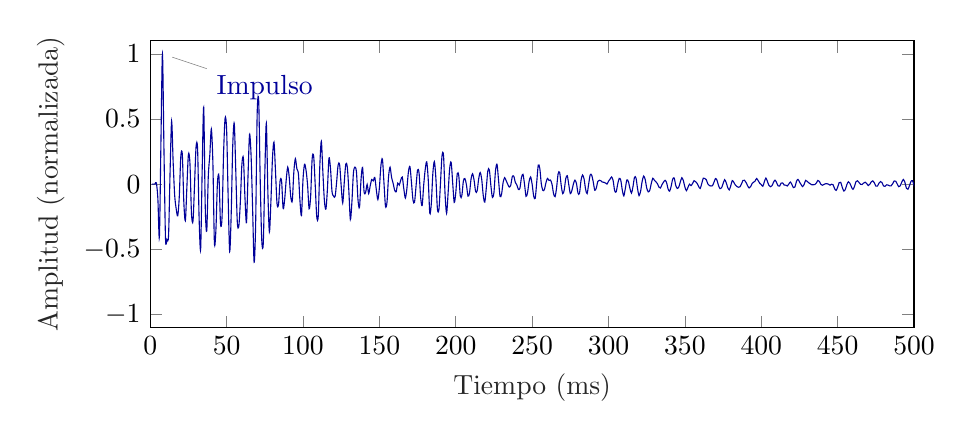
\begin{tikzpicture}

\begin{axis}[%
width=0.8\textwidth,
height=0.3\textwidth,
at={(0\textwidth,0\textwidth)},
scale only axis,
xmin=0,
xmax=500,
xlabel style={font=\color{white!15!black}},
xlabel={Tiempo (ms)},
ymin=-1.1,
ymax=1.1,
ylabel style={font=\color{white!15!black}},
ylabel={Amplitud (normalizada)},
axis background/.style={fill=white},
legend style={legend cell align=left, align=left, draw=white!15!black}
]
\addplot [color=black!40!blue, smooth]
  table[row sep=crcr]{%
1	4.2434738134034e-05\\
2	-0.000305107333076649\\
3	-7.00303905887267e-05\\
4	0.0102163738390573\\
5	-0.112658317720332\\
6	-0.406324005259592\\
7	0.31944440485853\\
8	1\\
9	0.254143471158102\\
10	-0.419421552342101\\
11	-0.426049295861048\\
12	-0.391400555358473\\
13	0.0981040777945736\\
14	0.483833119630901\\
15	0.168320936215935\\
16	-0.0859970762599573\\
17	-0.190508299724286\\
18	-0.243018733499582\\
19	-0.0987719084795913\\
20	0.210747821340874\\
21	0.227070515693981\\
22	-0.141382759360567\\
23	-0.280890280339065\\
24	-0.0190941612947313\\
25	0.229452560179539\\
26	0.158762720075231\\
27	-0.226287102827428\\
28	-0.282467801318148\\
29	-0.00503940027795124\\
30	0.287091012549922\\
31	0.269219668431788\\
32	-0.263795015217624\\
33	-0.499225118077277\\
34	0.105422543579266\\
35	0.589718130115671\\
36	-0.168493735741663\\
37	-0.359430073266253\\
38	0.0594348920738526\\
39	0.222884163049741\\
40	0.423905565786697\\
41	0.169746475134616\\
42	-0.448428448844936\\
43	-0.349434729393238\\
44	0.0100225795323468\\
45	0.0560272364984939\\
46	-0.303099856773429\\
47	-0.253889564060103\\
48	0.23234192057231\\
49	0.505904690192608\\
50	0.418494778447894\\
51	-0.0954006723407019\\
52	-0.517671052265655\\
53	-0.229571714919757\\
54	0.291956986380569\\
55	0.465429827611331\\
56	0.101402533289217\\
57	-0.293070159868023\\
58	-0.321418086440985\\
59	-0.133090839518047\\
60	0.151731987301162\\
61	0.197543487685493\\
62	-0.10130285321253\\
63	-0.29479540559754\\
64	0.0604133027735543\\
65	0.380137476085054\\
66	0.223202331101447\\
67	-0.179516539250699\\
68	-0.599675232169716\\
69	-0.307284551693044\\
70	0.540141287740539\\
71	0.640677984843933\\
72	0.0264150876811868\\
73	-0.429267349915847\\
74	-0.454558141731809\\
75	0.0755832132248315\\
76	0.466891775170438\\
77	-0.0590980872991054\\
78	-0.367175145091721\\
79	-0.131366219661402\\
80	0.194727338775749\\
81	0.322162139497323\\
82	0.098608302574462\\
83	-0.149886334811868\\
84	-0.154196905265678\\
85	0.0248283318823042\\
86	0.021645678888035\\
87	-0.187116275132325\\
88	-0.11650518990632\\
89	0.0310209873227905\\
90	0.130955914545893\\
91	0.0517600836509473\\
92	-0.0981347924997635\\
93	-0.126372322478858\\
94	0.0925800218392396\\
95	0.194798953188524\\
96	0.117775174148505\\
97	0.0783790449436879\\
98	-0.1251269770504\\
99	-0.240832472672594\\
100	0.035454599574507\\
101	0.152797575955049\\
102	0.105299456113073\\
103	-0.00706682739468079\\
104	-0.189611018476398\\
105	-0.0944133180597078\\
106	0.196586191451445\\
107	0.211804747862686\\
108	-0.00667469430374013\\
109	-0.249825265577499\\
110	-0.242687347408605\\
111	0.136721513472651\\
112	0.328828153139852\\
113	0.0944185448216786\\
114	-0.126003221017186\\
115	-0.191112373988062\\
116	-0.0350411528050927\\
117	0.199966879759643\\
118	0.119847114658569\\
119	-0.0572502811593267\\
120	-0.0910512073435825\\
121	-0.0958444684911797\\
122	0.0133702644259301\\
123	0.148101897439403\\
124	0.146651979151102\\
125	-0.0132571261748922\\
126	-0.144932274189273\\
127	0.010654652132871\\
128	0.153178028330387\\
129	0.130978914609784\\
130	-0.0476576428244471\\
131	-0.270963245458972\\
132	-0.140528094680974\\
133	0.0853112454921074\\
134	0.130835545676177\\
135	0.0924931284478134\\
136	-0.120051587045339\\
137	-0.177102480678457\\
138	0.0371928058235653\\
139	0.127959609110803\\
140	-0.0599990574245908\\
141	-0.0627313888408594\\
142	-0.00212402937717115\\
143	-0.0721876160693569\\
144	-0.0124906252990513\\
145	0.0360094308679209\\
146	0.0252631431896475\\
147	0.0518191336979612\\
148	-0.0437834827953338\\
149	-0.117981632034684\\
150	-0.0292763853273641\\
151	0.142005632885457\\
152	0.191068427242101\\
153	0.0103488200060156\\
154	-0.169699326082309\\
155	-0.137320382611392\\
156	0.0568251156432211\\
157	0.129417870705595\\
158	0.0506198407852594\\
159	0.00652463677499782\\
160	-0.0458751656890399\\
161	-0.0591677519568634\\
162	0.00738421650282817\\
163	-0.00703130163242349\\
164	0.0318282709056916\\
165	0.0543793011042908\\
166	-0.0362049096157193\\
167	-0.10651740675678\\
168	-0.0353479096588671\\
169	0.0942289376151848\\
170	0.134295257072552\\
171	0.0131625477971511\\
172	-0.121981508204044\\
173	-0.13952180224527\\
174	-0.0160694973783961\\
175	0.10877638555769\\
176	0.0832842033232737\\
177	-0.100431173229026\\
178	-0.164261877352033\\
179	-0.00954893336120222\\
180	0.112077588323132\\
181	0.171385583112794\\
182	0.0311299561038823\\
183	-0.222343604322589\\
184	-0.148974586548434\\
185	0.0824104242174712\\
186	0.172872288632277\\
187	0.042542604962307\\
188	-0.19106152633276\\
189	-0.192024428491607\\
190	0.0088846948834771\\
191	0.217461004554366\\
192	0.219072593677708\\
193	-0.0779842820162457\\
194	-0.223968732455035\\
195	-0.0664861343670395\\
196	0.118553378920581\\
197	0.166843463401449\\
198	0.00740557834018318\\
199	-0.14071526386698\\
200	-0.0671892564222389\\
201	0.0817634534168974\\
202	0.0617557646910996\\
203	-0.0930417383475515\\
204	-0.0865978131771499\\
205	0.0255189855460003\\
206	0.0431554407566068\\
207	-0.00604058857481959\\
208	-0.0918091074512972\\
209	-0.0682941217426674\\
210	0.0393914200984682\\
211	0.0791040166041626\\
212	0.030301662908073\\
213	-0.056136602907543\\
214	-0.0523983151060747\\
215	0.0409561999382504\\
216	0.0891191952794657\\
217	0.0365043645761034\\
218	-0.0875616848279606\\
219	-0.137852253356471\\
220	-0.0284548843452512\\
221	0.103078385620734\\
222	0.107949878982652\\
223	-0.0120350665206388\\
224	-0.102279367961046\\
225	-0.0635638457451932\\
226	0.100496370789642\\
227	0.15274070862705\\
228	0.0311269755749777\\
229	-0.0946517995159297\\
230	-0.0752682551755015\\
231	0.0128846884498444\\
232	0.0498888132935917\\
233	0.026360005551453\\
234	7.79022378196714e-05\\
235	-0.0223584443212985\\
236	-0.00766427103712886\\
237	0.0570655790829733\\
238	0.0601808020367116\\
239	0.0137279947801972\\
240	-0.00673958175144662\\
241	-0.0403883228201494\\
242	-0.031348045933953\\
243	0.0503081724390881\\
244	0.0754672687799598\\
245	0.00087901105786159\\
246	-0.0938608516431714\\
247	-0.0644502895835899\\
248	0.0201143367866052\\
249	0.0550681791359011\\
250	-0.000619648405461248\\
251	-0.0909182481454422\\
252	-0.109153313949321\\
253	0.0137708880162108\\
254	0.145882386525614\\
255	0.122049615755884\\
256	0.00266680473629322\\
257	-0.0477137107558292\\
258	-0.0419497184457214\\
259	0.00873475663888712\\
260	0.0437470401822679\\
261	0.0289364715410443\\
262	0.03151162024011\\
263	-0.000538120093835914\\
264	-0.0719918758077256\\
265	-0.0964718927539252\\
266	-0.0274812659419013\\
267	0.0794381606846173\\
268	0.0902784969155732\\
269	-0.00619325750631106\\
270	-0.0728387356438702\\
271	-0.0452518729547364\\
272	0.0415065693133556\\
273	0.0647258425048562\\
274	-0.00500829681197956\\
275	-0.0725999222960354\\
276	-0.0497784352866688\\
277	0.000752310835082426\\
278	0.0307166094751778\\
279	0.00608676545988374\\
280	-0.0681502048426523\\
281	-0.0700930929307333\\
282	0.029321406867723\\
283	0.0706052350790287\\
284	0.0393160388475735\\
285	-0.0401512793812913\\
286	-0.0724919350228106\\
287	0.00136660403484257\\
288	0.0712012199193168\\
289	0.0688434313006496\\
290	0.0172088426002119\\
291	-0.0469553445916517\\
292	-0.029606205441894\\
293	0.021024349888819\\
294	0.0297822344522842\\
295	0.0258182686042119\\
296	0.015424765639068\\
297	0.014596340932826\\
298	0.00854085178730202\\
299	0.000487765415982722\\
300	0.0228182881962766\\
301	0.0384994666932243\\
302	0.0552011899724789\\
303	0.0285647467799208\\
304	-0.049585522189318\\
305	-0.0596867280301012\\
306	0.000432778744880125\\
307	0.0445485189810029\\
308	0.0309135697626743\\
309	-0.0447182628378187\\
310	-0.090275082360165\\
311	-0.0331579162024127\\
312	0.0323299779940953\\
313	0.0196934447252488\\
314	-0.0316931331243495\\
315	-0.0688494380389102\\
316	-0.0200748759817202\\
317	0.052034527963599\\
318	0.0469639463611315\\
319	-0.0351958955350824\\
320	-0.0880734492340025\\
321	-0.0549242532201788\\
322	0.0202141360426822\\
323	0.0622289245903858\\
324	0.0358012238015704\\
325	-0.029819710380707\\
326	-0.0594779626476338\\
327	-0.0468180682967727\\
328	0.00577341752273242\\
329	0.0454326824394684\\
330	0.0304994112390773\\
331	0.0181471727007079\\
332	0.00415997360016718\\
333	-0.0230774475172097\\
334	-0.0301258992751627\\
335	-0.00351817480367345\\
336	0.0154935559578462\\
337	0.0293805509508047\\
338	0.0113993348299459\\
339	-0.037433231509965\\
340	-0.0539008479468635\\
341	-0.0161484505050566\\
342	0.0379783335305319\\
343	0.046785150784217\\
344	-0.00953691376133747\\
345	-0.0330822481678297\\
346	-0.0217303835157736\\
347	0.0172780419010792\\
348	0.0489747692393507\\
349	0.0265602932822162\\
350	-0.0225584975509037\\
351	-0.0501717989228041\\
352	-0.0247803080171138\\
353	-0.000209979310739072\\
354	-0.0111520710445348\\
355	0.00512303188395435\\
356	0.0264969893882494\\
357	0.0194849907384764\\
358	0.00548351648365042\\
359	-0.0177614956663774\\
360	-0.0332959888409619\\
361	0.00334742723680392\\
362	0.0452125599201167\\
363	0.0445468702614562\\
364	0.0336247824390057\\
365	0.00236398909515856\\
366	-0.0108177590376499\\
367	-0.0144012044676174\\
368	-0.012004745096533\\
369	0.0132066533295756\\
370	0.0429041146734335\\
371	0.0302277118415759\\
372	-0.0104773394855897\\
373	-0.0344542568789734\\
374	-0.0283710367054937\\
375	0.00400111953985061\\
376	0.034041053394958\\
377	0.0123562573841696\\
378	-0.0248798930180101\\
379	-0.0443324328667245\\
380	-0.0127007652255884\\
381	0.0274987306607954\\
382	0.0142068308153398\\
383	-0.00674589324421504\\
384	-0.0178977607682214\\
385	-0.0236760189014262\\
386	-0.0208664813910673\\
387	0.000318765237182106\\
388	0.0280427069447455\\
389	0.0298899829273864\\
390	0.0135987779480615\\
391	-0.0113421737564749\\
392	-0.0292236855831334\\
393	-0.0196050863545452\\
394	0.00513004241508952\\
395	0.0152305783949487\\
396	0.0241923885324127\\
397	0.0430875755562283\\
399	0.00650351434666163\\
400	-0.00390418419073058\\
401	-0.0163808607109104\\
402	0.0179660765792278\\
403	0.0468076039156244\\
404	0.0215092558023571\\
405	-0.00962535935826736\\
406	-0.019784575810661\\
407	-0.0124071416098559\\
408	0.0140352926419496\\
409	0.0304130267627443\\
410	0.012113601805936\\
411	-0.0134811746702894\\
412	-0.0145640678023824\\
413	0.00781262337699218\\
414	0.0093014204472297\\
415	-0.0067624452000814\\
416	-0.00745235216993478\\
417	-0.0143150791455469\\
418	0.00021101377302557\\
419	0.0164046855479683\\
420	-0.00158481591853388\\
421	-0.0264223996583155\\
422	-0.0225696346008135\\
423	0.0195210931047427\\
424	0.036884017318016\\
425	0.0169647835085129\\
426	-0.0019110640969302\\
427	-0.0185311580900702\\
428	-0.00363193338785095\\
429	0.02889931526704\\
430	0.0223407891387524\\
431	0.0112897203297848\\
433	-0.00441399808357801\\
434	-0.00468176819299515\\
435	-0.00311968028154297\\
436	0.00758816342113278\\
437	0.0281175924312151\\
438	0.0211610488794349\\
439	-0.000960052333766725\\
440	-0.00879715557852023\\
441	-0.00235846747290225\\
442	0.00282371777643675\\
443	0.00376019462129307\\
444	-0.000503929943477033\\
445	-0.00782279681783393\\
446	-0.000737570513990704\\
447	-0.00475165581065085\\
448	-0.0347967952396289\\
449	-0.0481855300386655\\
450	-0.0228921351777558\\
451	0.0116004779522996\\
452	0.0141549879012928\\
453	-0.0240395930988484\\
454	-0.0527800368865883\\
455	-0.0404179472573674\\
456	-0.00434876993614353\\
457	0.0180017840324922\\
458	0.00691907349289522\\
459	-0.021053907509895\\
460	-0.0398426040100048\\
461	-0.0178982621434329\\
462	0.0201176878541673\\
463	0.0258475057381133\\
465	-0.00176443867593434\\
466	-0.00247937028404976\\
467	0.00824667609805374\\
468	0.014986121715026\\
469	0.00427453796714872\\
470	-0.0105766838909176\\
471	-0.00149741030219275\\
472	0.017347225648507\\
473	0.0251093065790542\\
474	0.0110516863589964\\
475	-0.0155704175779761\\
476	-0.0152816398357345\\
477	0.0064252181913389\\
478	0.0195429751263418\\
479	0.0130065196967166\\
480	-0.0136514029958335\\
481	-0.017260731840679\\
482	-0.00500913717536378\\
483	-0.00696824345953928\\
484	-0.0129316154050798\\
485	-0.0130602274383023\\
486	0.00336729786306478\\
487	0.0243823891437955\\
488	0.0223730838646929\\
489	0.00112983178507875\\
490	-0.0195751815114136\\
491	-0.0128517940416941\\
492	0.0168775608927376\\
493	0.0360479266161633\\
494	0.0140244759079451\\
495	-0.0315260872309864\\
496	-0.0394578507611527\\
497	-0.0115326535533882\\
498	0.0206041748820098\\
499	0.026745505363408\\
500	-0.00948803025585221\\
501	-0.0346936412250898\\
};
\addplot[mark=none, color=black!40!blue] coordinates {(8,1)} node[pin=-15:{Impulso}]{} ;

\end{axis}
\end{tikzpicture}%
    }
    \caption{Respuesta al impulso de un sistema.}
    \label{graf:impulso}
\end{figure}





